% To familiarize yourself with this template, the body contains
% some examples of its use.  Look them over.  Then you can
% run LaTeX on this file.  After you have LaTeXed this file then
% you can look over the result either by printing it out with
% dvips or using xdvi. "pdflatex template.tex" should also work.
%

\documentclass[oneside]{article}
\setlength{\oddsidemargin}{0.25 in}
\setlength{\evensidemargin}{-0.25 in}
\setlength{\topmargin}{-0.6 in}
\setlength{\textwidth}{6.5 in}
\setlength{\textheight}{8.5 in}
\setlength{\headsep}{0.75 in}
\setlength{\parindent}{0 in}
\setlength{\parskip}{0.1 in}

%
% ADD PACKAGES here:
%

\usepackage{caption}
\usepackage{subfig}
\usepackage{amsmath,amsfonts,graphicx,algorithmic,algorithm}

%
% The following commands set up the lecnum (lecture number)
% counter and make various numbering schemes work relative
% to the lecture number.
%
\newcounter{lecnum}
\renewcommand{\thepage}{\thelecnum-\arabic{page}}
\renewcommand{\thesection}{\arabic{section}}
\renewcommand{\theequation}{\thelecnum.\arabic{equation}}
\renewcommand{\thefigure}{\thelecnum.\arabic{figure}}
\renewcommand{\thetable}{\thelecnum.\arabic{table}}

%
% The following macro is used to generate the header.
%
\newcommand{\lecture}[4]{
   \pagestyle{myheadings}
   \thispagestyle{plain}
   \newpage
   \setcounter{lecnum}{#1}
   \setcounter{page}{1}
   \noindent
   \begin{center}
   \framebox{
      \vbox{\vspace{2mm}
    \hbox to 6.28in { {\bf 18660 Project Final Report
	\hfill 10 May 2018} }
       \vspace{7mm}
       \hbox to 6.28in { {\Large \hfill Comparison of robust PCA techniques in image and video processing  \hfill} }
       \vspace{4mm}
       \hbox to 6.28in { {\hfill\it Joel Loo, Wang Xueqiang \hfill} }
      \vspace{2mm}}
   }
   \end{center}
   \markboth{Project Final Report}{Project Final Report}

   %{\bf Note}: {\it LaTeX template courtesy of UC Berkeley EECS dept.}
   %vspace*{4mm}
}
%
% Convention for citations is authors' initials followed by the year.
% For example, to cite a paper by Leighton and Maggs you would type
% \cite{LM89}, and to cite a paper by Strassen you would type \cite{S69}.
% (To avoid bibliography problems, for now we redefine the \cite command.)
% Also commands that create a suitable format for the reference list.
\renewcommand{\cite}[1]{[#1]}
\def\beginrefs{\begin{list}%
        {[\arabic{equation}]}{\usecounter{equation}
         \setlength{\leftmargin}{2.0truecm}\setlength{\labelsep}{0.4truecm}%
         \setlength{\labelwidth}{1.6truecm}}}
\def\endrefs{\end{list}}
\def\bibentry#1{\item[\hbox{[#1]}]}

%Use this command for a figure; it puts a figure in wherever you want it.
%usage: \fig{NUMBER}{SPACE-IN-INCHES}{CAPTION}
\newcommand{\fig}[3]{
			\vspace{#2}
			\begin{center}
			Figure \thelecnum.#1:~#3
			\end{center}
	}
% Use these for theorems, lemmas, proofs, etc.
\newtheorem{theorem}{Theorem}[lecnum]
\newtheorem{lemma}[theorem]{Lemma}
\newtheorem{proposition}[theorem]{Proposition}
\newtheorem{claim}[theorem]{Claim}
\newtheorem{corollary}[theorem]{Corollary}
\newtheorem{definition}[theorem]{Definition}
\newenvironment{proof}{{\bf Proof:}}{\hfill\rule{2mm}{2mm}}

% **** IF YOU WANT TO DEFINE ADDITIONAL MACROS FOR YOURSELF, PUT THEM HERE:

\newcommand\E{\mathbb{E}}
\newcommand{\compconj}[1]{%
  \overline{#1}%
}

\begin{document}
%FILL IN THE RIGHT INFO.
%\lecture{**LECTURE-NUMBER**}{**DATE**}{**LECTURER**}{**SCRIBE**}
\lecture{1}{0}{1}{Joel Loo, Wang Xueqiang}
\section{Introduction}
Principal components analysis (PCA) and other dimensionality reduction techniques have gained wide traction in the scientific community because of their utility in extracting salient data from large and complex datasets. However, PCA implicitly assumes that the noise in data is small and variance from the mean is bounded (such as in Gaussian noise), causing it to perform poorly on grossly corrupted data, or data containing outliers of significant magnitude.\newline\newline
While there have been many attempts to robustify PCA, many of these methods are heuristics without any optimality guarantees. However, recent advances in low-rank matrix recovery and completion by Candes et al [1], have led to the formulation of robust PCA (RPCA). In RPCA, the problem is reformulated as the recovery of the matrices $L, S$ such that $M = L + S$, where $M$ is the original matrix, $L$ is a low-rank matrix and $S$ is a sparse matrix. Candes et al made the surprising observation that it is possible to perform this decomposition through a tractable convex optimization, if we assume that the low-rank matrix is not simultaneously sparse [1]. In particular, this can be achieved using the Principal Component Pursuit (PCP) estimate which solves the problem
\begin{center}
$
\begin{aligned}
& \underset{L,S}{\text{argmin}}
& & \lVert L\rVert_{*}+ \lambda\lVert S\rVert_{1} 
& \text{subject to}
& & L+S=M
\end{aligned}
$
\end{center}
Since the sparse matrix can have elements of arbitrarily large magnitude, robust PCA thus improves over the PCA technique by allowing the extraction of low-dimensional structure from grossly corrupted data with unbounded outliers. This technique has many important applications in general, and in particular is of great utility in computer vision, where it is used in tackling problems such as background recovery/subtraction (which can be used in video surveillance software), removal of non-Lambertian distortions/specularities/shadows from images (akin to performing inpainting) and even recovery of 3D geometry from low-rank textures in 2D images.\newline\newline
In order to make RPCA practicable on real-world vision systems, a number of reformulations of the problem and improvements have been proposed. Some of these improvements (e.g. Fast PCP [3]) provide significant speed improvements over the method proposed by Candes et al, while others reformulate RPCA as an online algorithm (e.g. online RPCA via stochastic optimization [2], iFrALM).
\section{Problem Statement}
In this project, we aim to survey several RPCA algorithms - in particular we will implement these algorithms and compare their performance, in terms of both speed and ability to separate low-rank structure from sparse noise. We are primarily interested in applying these algorithms to, and testing them on vision applications. Two applications that we are particularly interested in are the removal of specularities/non-Lambertian distortions from images, as well as background recovery/subtraction in videos. Background recovery/subtraction in video streams provides an interesting case study for RPCA as well, since it is desirable to have both algorithms that can separate backgrounds in post-processing as well as on the fly. To this end, we will use this particular application to benchmark the performance of both RPCA algorithms that offer significant speed-ups, as well as RPCA algorithms formulated to be online in nature. We will perform the implementations and benchmarking described above in Python, with code available on the private Github repository https://github.com/joelloo/18660\_project
\section{Methods}
In this section, we discuss the formulation of the optimization problems for the various algorithms and our approach to their implementation. As mentioned, we are implementing these algorithms with an eye toward applying them on specularity removal from Lambertian surfaces and realtime background subtraction in video streams. The low-rank/sparse decomposition is relevant in specularity removal from images, since convex-shaped Lambertian objects can generally be approximated by a low dimensional linear subspace [11, 12]. As such, running RPCA on scenes containing objects that can be approximated by convex-shaped Lambertian surfaces cannot allow us to separate distortions such as specularities and occlusions from the scene. With regards to background subtraction in video streams, RPCA is relevant since we can vectorize each frame of the stream and concatenate them to form a matrix. This matrix can then be modelled as the sum of a low-rank matrix, which represents the background (i.e. all that is constant across frames), and the sparse matrix, which represents the movements in the foreground of the image. Hence, the low-rank/sparse decomposition can allow us to separate background and foreground in video streams.\newline\newline
We make the distinction between offline and online RPCA algorithms, i.e. algorithms that require the entire matrix beforehand to perform the low-rank/sparse decomposition as opposed to algorithms that can take in new columns of the matrix as they come in and update the decomposition on the fly. In particular, online RPCA algorithms allow us to perform realtime background subtraction, where we have an online setting with new frames coming in from the video stream.
\subsection{Offline RPCA Algorithms}
The original PCP formulation of the RPCA algorithm  has several immediately apparent solutions. We can consider the relaxation $\underset{L,S}{\text{argmin}} \lVert L\rVert_{*} + \lVert S\rVert_{1} + \frac{1}{2}\lVert M-L-S\rVert^{2}_{F}$. Since $\lVert\cdot\rVert_{*}$ and $\lVert\cdot\rVert_{1}$ have well-known proximal operators in the singular value thresholding operator [9] and the soft thresholding operator, while $\lVert\cdot\rVert_{F}$ is differentiable, it is clear that we can solve this formulation via proximal gradient descent. Indeed, Lin et al. [5] provide an accelerated proximal gradient descent (APG) based algorithm that solves this formulation by alternately minimizing $L$ (with singular value thresholding) then $E$ (with soft thresholding) at each iteration.\newline\newline
Another possible means of approaching the PCP formulation is via the augmented Lagrangian multiplier method (ALM), as suggested by Candes et al. in [1] and elaborated on by Lin et al. in [8]. We can write the Lagrangian function of the PCP formulation as $\mathcal{L}(L,S, Y, \mu) = \lVert L\rVert_{*} + \lambda\lVert S\rVert_{1} + \langle Y, M-L-S\rangle +\frac{\mu}{2}\lVert M-L-S\rVert_{F}^{2}$.
\begin{algorithm}
 \caption{Augmented Lagrangian multiplier method}
 \begin{algorithmic}  
 \STATE Initialize $Y_{0} = sgn(D)/J(sgn(D)$; $\mu_{0} >0$; $\rho > 1$; $k = 0$
\WHILE{not converged}
\STATE $(L_{k+1}^{*}, S_{k+1}^{*}) = \underset{L,S}{\text{argmin   }}\mathcal{L}(L,S,Y_{k}^{*},\mu_{k})$
\STATE $Y_{k+1}^{*} = Y_{k}^{*} + \mu_{k}(M-L_{k+1}^{*}-S_{k+1}^{*})$
\STATE Update $\mu_{k}$ to $\mu_{k+1}$
\ENDWHILE
\RETURN $L_{k}, S_{k}$
 \end{algorithmic}
 \end{algorithm}\newline
The augmented Lagrangian multiplier algorithm takes the approach described in algorithm 1. In order to perform the minimization of $\mathcal{L}$ wrt $L, S$, we can perform an alternating minimization where we first update $L_{k+1}$ (using singular value thresholding) and then $S_{k+1}$ (using soft thresholding), similar to APG. We can perform this until convergence, to obtain $L_{k+1}^{*}, S_{k+1}^{*}$. In contrast to this exact ALM approach, Lin et al. also proposed an inexact ALM approach, wherein the minimization of $\mathcal{L}$ is simply replaced by one iteration of the alternating minimization approach (i.e. a single singular value thresholding and soft thresholding step). This can be proved to converge to the optimal value, while doing less work by removing the nested loop [8]. This is referred to as the inexact ALM approach, since we are not solving exactly for $L_{k+1}^{*}, S_{k+1}^{*}$.\newline\newline
A major difficulty in implementing inexact ALM as described by Candes et al. lay in the initialization of $Y_{0}$. Our algorithm with a randomly initialized $Y_{0}$ did not perform as well as the results from studies implementing inexact ALM. However, Lin et al. suggest the usage of the initializer $Y_{0} = sgn(D)/J(sgn(D))$ where $J = \max\{\lVert\cdot\rVert_{2},\lVert\cdot\rVert_{\infty}\}$, which ensures that $\langle D,Y_{0}\rangle$ is a reasonably large value to begin with [8], thereby speeding convergence.\newline\newline
We also considered the Fast PCP algorithm [3]. In contrast to the previous approaches, Fast PCP relaxes the constraint $M=L+S$ to a penalty in the objective function while also transforming the nuclear norm penalty into the constraint $\lVert L\rVert_{*}\le t$. Rodriguez et al. argue that in practice we are mainly interested in solutions for which this constraint is active, i.e. $\lVert L\rVert_{*} = t$. Considering only this case, we can express the nuclear norm equality constraint directly as a rank constraint, i.e. rank$(L) \le t$. This yields the problem $$
\begin{aligned}
& \underset{L,S}{\text{argmin}}
& & \lVert L+S-M\rVert_{F}+ \lambda\lVert S\rVert_{1} 
& \text{subject to}
& & \text{rank}(L) = t
\end{aligned}
$$
We recognize that this problem is amenable to alternating minimization, since it comprises the sub-problems\newline
$\begin{cases}
L_{k+1}  =\begin{aligned}
& \underset{L}{\text{argmin}}
& & \lVert L_{k}+S_{k}-M\rVert_{F}
& \text{subject to}
& & \text{rank}(L_{k}) = t
\end{aligned}\\
S_{k+1} = \begin{aligned}
& \underset{S}{\text{argmin}}
& & \lVert L_{k+1}+S_{k}-M\rVert_{F}+ \lambda\lVert S\rVert_{1} 
\end{aligned}
\end{cases}
$\newline
We recognize the first sub-problem as a rank-constrained least squares problem, for which the canonical solution is to compute the partial SVD of $M-S$ up to rank $t$. The second sub-problem is similar in form to LASSO and can be solved by direct application of the soft thresholding operator.\newline\newline
The algorithm derived from this reformulation of the PCP objective is remarkably simple. To compute the partial SVD, we used scikit-learn's $randomized\_svd$ function to efficiently compute the SVD up to the estimated rank. As suggested in [3], we also implemented a heuristic check to enforce low rank in $L$, wherein we compute the contribution of each successive singular value, and stop increasing the rank when the singular value becomes too small. Since the soft thresholding step is not computationally expensive, and the cost of computing the SVD is heavily mitigated since we are only computing the partial SVD up to a low rank, this algorithm is computationally cheap and thus fast.
\subsection{Online RPCA Algorithms}
An online algorithm adapted to process video streams on the fly has to be able to take in new frames, and has to have a mechanism for adding new frames to the matrix of vectorized frames and updating the decomposition. These are not features the previous algorithms possess, precluding them from use as true online algorithms.
We first consider incremental stochastic RPCA (STOC-RPCA) [2]. This algorithm adapts the original PCP formulation, relaxing the $M=L+S$ constraint as a penalty in the objective and 
expressing the nuclear norm as $\inf\limits_{L,R}\{\frac{1}{2}\lVert L\rVert_{F}^{2} +\frac{1}{2}\lVert R\rVert_{F}^{2}: X = LR^{T}\}$, where $L$ can be thought of as a fixed basis. Substituting this back into objective expression and converting into a form that takes each column vector of $R$ and $S$ (corresponding to each video frame) as arguments, we have $\frac{1}{t}\sum_{i=1}^{t}(\frac{1}{2}\lVert \textbf{m}_{i} - L\textbf{r}_{i} - \textbf{s}_{i}\rVert_{2}^{2} +\frac{\lambda_{1}}{2}\lVert \textbf{r}_{i}\rVert^{2}_{2} +\lambda_{2}\lVert \textbf{s}_{i}\rVert_{1}) + \frac{\lambda_{1}}{2t}\lVert L\rVert_{F}^{2}$. This can be solved through a alternating minimization, where we first minimize the objective with respect to $\textbf{r}_{i}$ and $\textbf{s}_{i}$, then update the basis $L$ using these vectors.\newline\newline
The paper recommended solving the first sub-problem to find $\textbf{r}_{i}, \textbf{s}_{i}$ using standard solvers. Since the first sub-problem is a convex problem, we attempted to use CVXPY to minimize the first sub-problem. This approach yielded poor results for reasons which we do not fully understand. However, a closer inspection showed that CVXPY was applying the ECOS solver for SOCPs to our problem. This sub-problem resembles a QP more than an SOCP, and we surmise that applying another solver more suited for QPs might resolve this issue. Our final solution to the first sub-problem was to take an alternating minimization approach, first updating $\textbf{r}_{i}$ and then updating $\textbf{s}_{i}$. The objective is fully differentiable with respect to $\textbf{r}_{i}$ and we can simply use the closed-form partial derivative to minimize for given $\textbf{s}_{i}$. The objective with respect to $\textbf{s}_{i}$ has the form of LASSO, and the minimizer of $\textbf{s}_{i}$ given $\textbf{r}_{i}$ for this iteration is given by the soft thresholding operator. Once we have computed $\textbf{r}_{i}, \textbf{s}_{i}$, we can update the basis $L$ using coordinate descent as suggested in [2]. Experiments indicate that this approach has good convergence properties, and yields acceptable results in a fairly fast.\newline\newline
Aside from this, we also implemented Incremental Fast PCP [10], a modification of the Fast PCP algorithm to turn it into an online algorithm. While the formulation of the optimization problem remains the same, the algorithm is modified to accommodate a constant incoming stream of video frames. Since the soft thresholding operator is an elementwise operator, it does not need to be modified for the online algorithm. For the partial SVD step however, the matrix has to be updated along with the SVD. Rodriguez et al. propose a method making use of the following SVD update functions, 
\begin{itemize}
\item Update: compute $U_{1}\Sigma_{1}V_{1}^{T} = [D \textbf{ d}]$ given $U_{0}\Sigma_{0}V_{0}^{T} = D$ and new frame \textbf{d}
\item Replace: compute $U_{1}\Sigma_{1}V_{1}^{T} = [D \text{ }\hat{\textbf{d}}\text{ } E]$ given $U_{0}\Sigma_{0}V_{0}^{T} = [D \textbf{ d } E]$ and modified frame $\hat{\textbf{d}}$
\item Downdate: compute $U_{1}\Sigma_{1}V_{1}^{T} = D$ given $U_{0}\Sigma_{0}V_{0}^{T} = [D \textbf{ d}]$
\end{itemize}
Recall that the partial SVD step takes the SVD of $M-S$ up to rank $t$. Given a new frame \textbf{m}, we can use the update function to find the SVD of the matrix $[M-S\textbf{ m}]$. We want to obtain the partial SVD of $[M-S \textbf{ m-s}]$. To do this, we can perform several iterations of alternating minimization on $L_{k}, S_{k}$ using the decomposition of the initial updated matrix $[M-S\textbf{ m-s}]$, using the partial SVD and soft thresholding operator as described in Fast PCP. Once we have converged on a better estimate of the sparse component $S$, we can use the replace operation to find the decomposition of $[M-S\textbf{ m-s}]$ instead, where \textbf{s} is the updated sparse component for the new frame \textbf{m}. In addition, Rodriguez et al. suggest the use of the downdating operation to remove earlier frames and maintain a sliding window of frames in the matrix $M$.\newline\newline
The workhorses of this algorithm are the SVD update operations, and we spent a significant amount of time understanding, implementing and testing for these operations for correctness. Brand [13] gives a concise description of how to implement rank-1 modifications for the SVD that allow us to achieve all 3 of the required SVD update operations listed above. In particular, these update algorithms allow us to compute a rank $r$ partial SVD in linear time, i.e. $O(pqr)$ for a matrix of size $p\times q$ and rank $r$, where columns of data are being streamed in to the matrix. Aside from the modifications needed to make the algorithm suitable for streaming data, and to make use of the SVD update operations, the implementation of Incremental Fast PCP remains similar in spirit to the implementation of Fast PCP.
\section{Results and comparisons}
We analyze and compare the performance of offline and online RPCA algorithms separately. We explore the performance in terms of the goodness of separation of low-rank and sparse components of an image or video stream, as well as the runtime performance of the various algorithms.
\subsection{Offline RPCA Algorithms}
\begin{figure}[ht]   
\centering
\subfloat[Specularity removal]{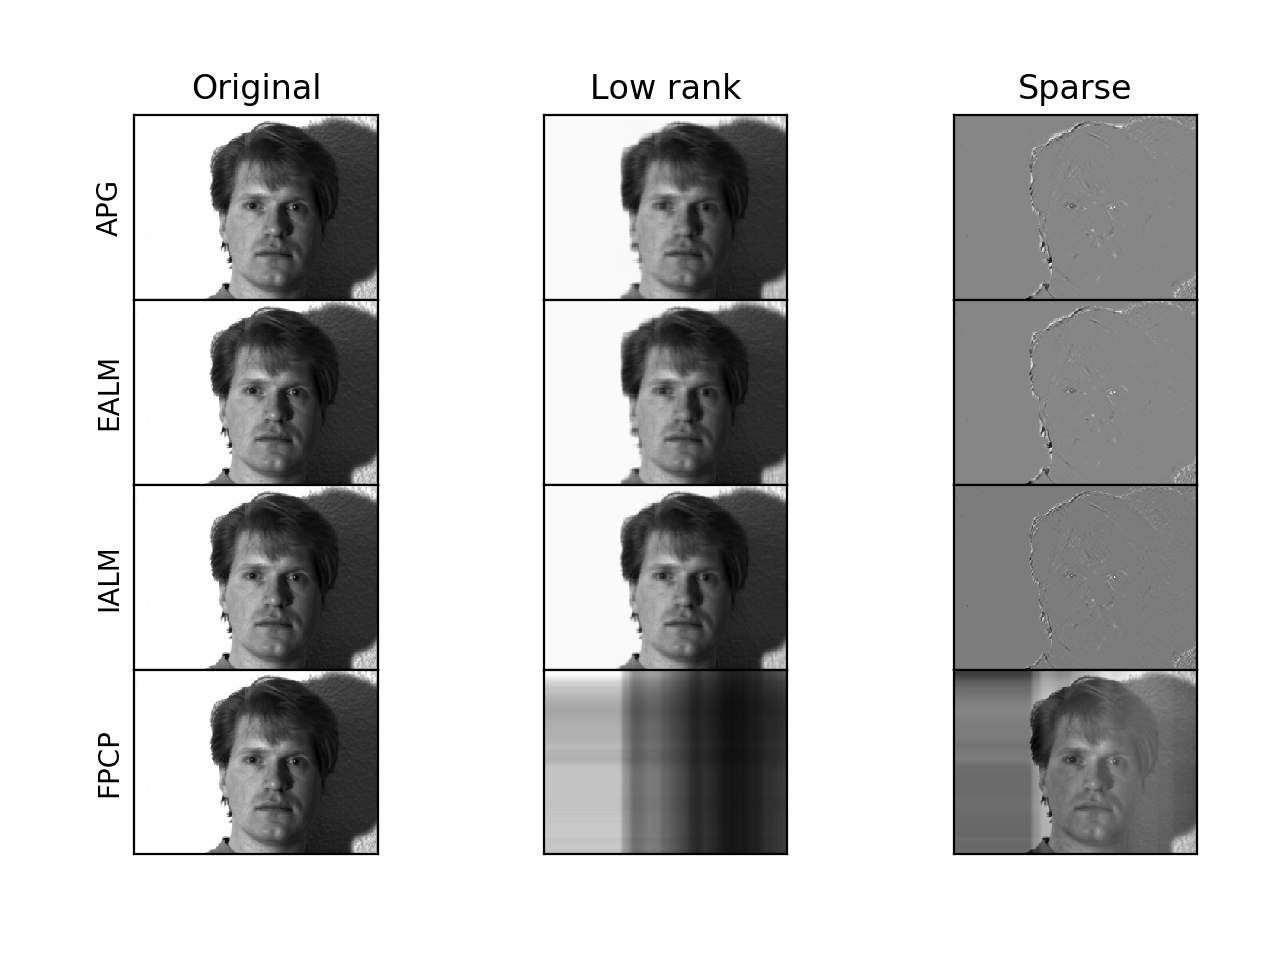
\includegraphics[width=0.5\textwidth, keepaspectratio]{Figure_1}\label{fig:subfig0}}
\subfloat[Video background subtraction]{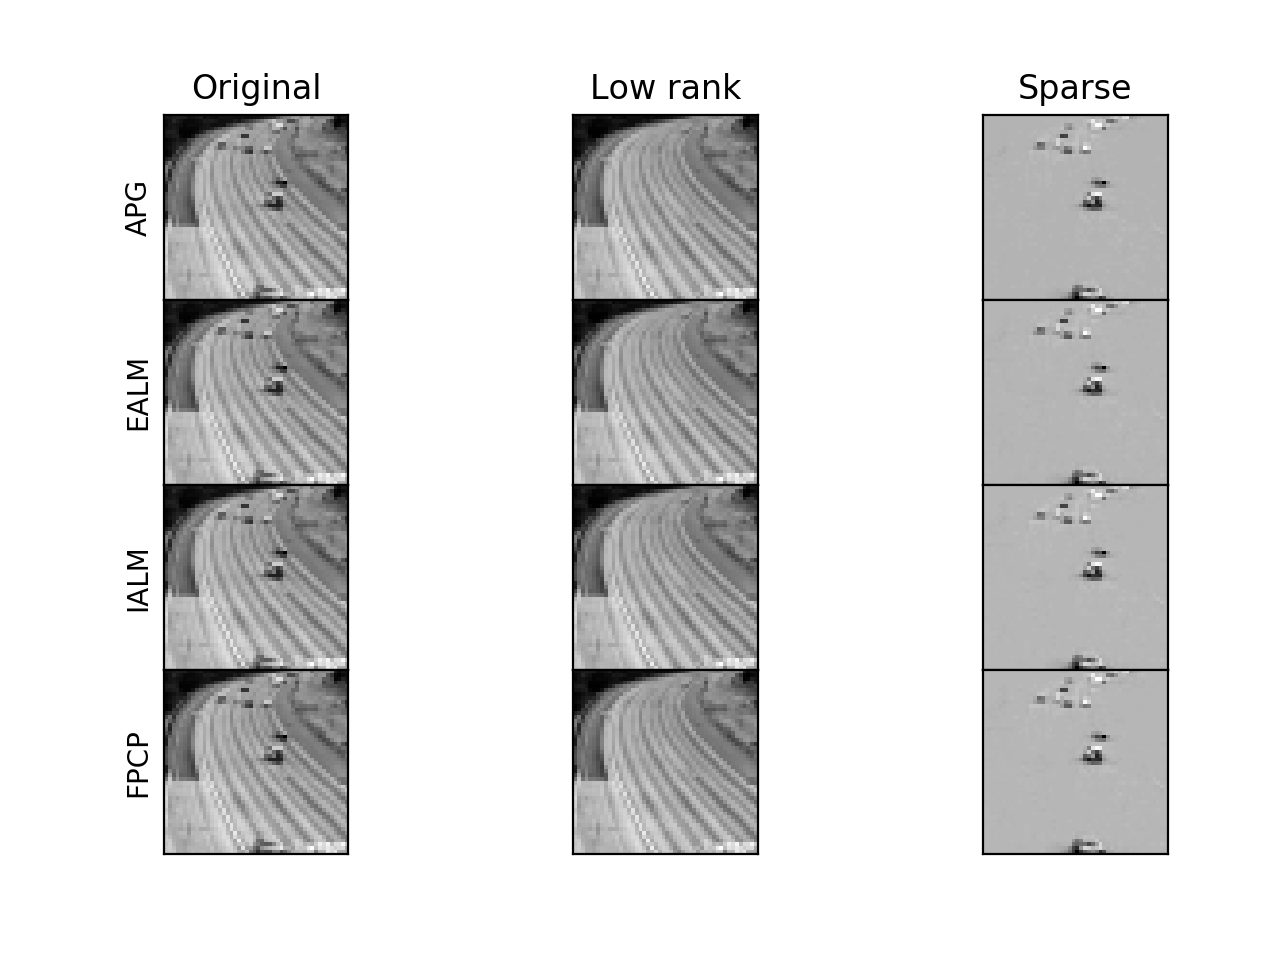
\includegraphics[width=0.5\textwidth, keepaspectratio]{Figure_2}\label{fig:subfig1}}
\caption[]{Performance of offline RPCA algorithms on image/video processing}
\label{fig:subfigureExample1}
\end{figure}
We benchmarked the performance of our offline RPCA algorithms by running them on specularity removal and background subtraction for videos. The human face under varying illumination can be approximated as a Lambertian surface, i.e. it lies close to a low-dimensional linear subspace, hence allowing us to directly apply RPCA to separate specularities from images of faces. Hence, we chose to run specularity removal tests on images from the YaleFaces database. For the video background subtraction tasks, we ran our algorithms on datasets from [14].\newline\newline
Fig. 1.1(a) shows an image from YaleFaces (with subject under left-aligned lighting) separated into low-rank and sparse components using the various offline RPCA algorithms implemented. We observe that APG, exact ALM and inexact ALM yield good results, with specularly reflected light in the subject's hair and eyes separated into the sparse component. Fast PCP yields visually undesirable results because it makes use of a heuristic that tends to prefer extremely low ranks for the low-rank matrix. The low-rank component separated is therefore of too low a rank to capture sufficient information about the subject's face. This heuristic however, works well on the video background subtraction task, where the rank of the vectorized collection of frames is indeed extremely low. This is evident through the excellent performance of Fast PCP in separating the moving cars from the background. We also observe similarly good performance from APG, exact and inexact ALM on the highway dataset.\newline\newline

\subsection{Online RPCA Algorithms}
\begin{figure}[ht]
\centering
\subfloat[STOC-RPCA]{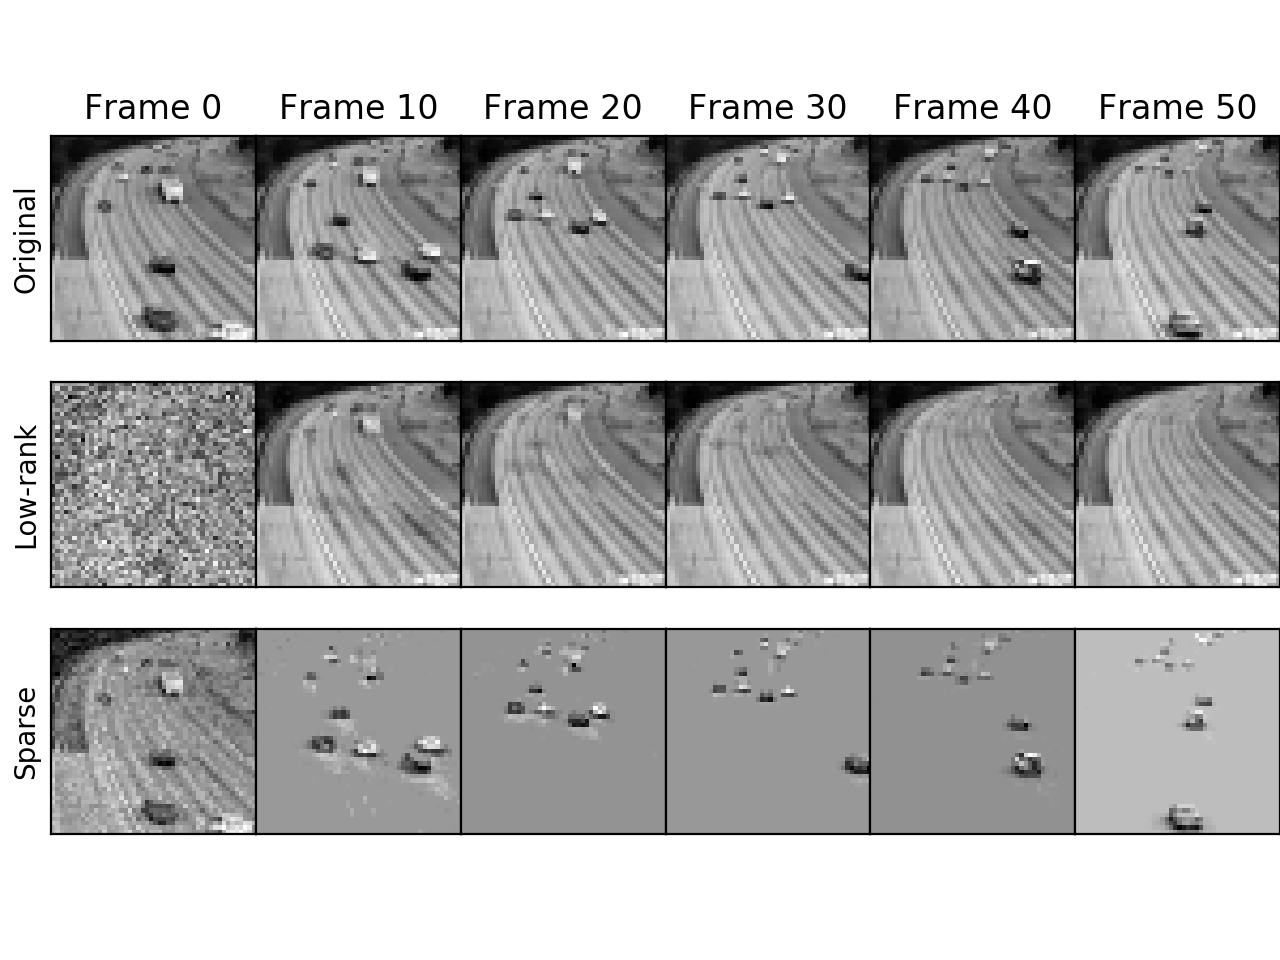
\includegraphics[width=0.5\textwidth, keepaspectratio]{Figure_3}\label{fig:subfig3}}
\subfloat[Incremental Fast PCP]{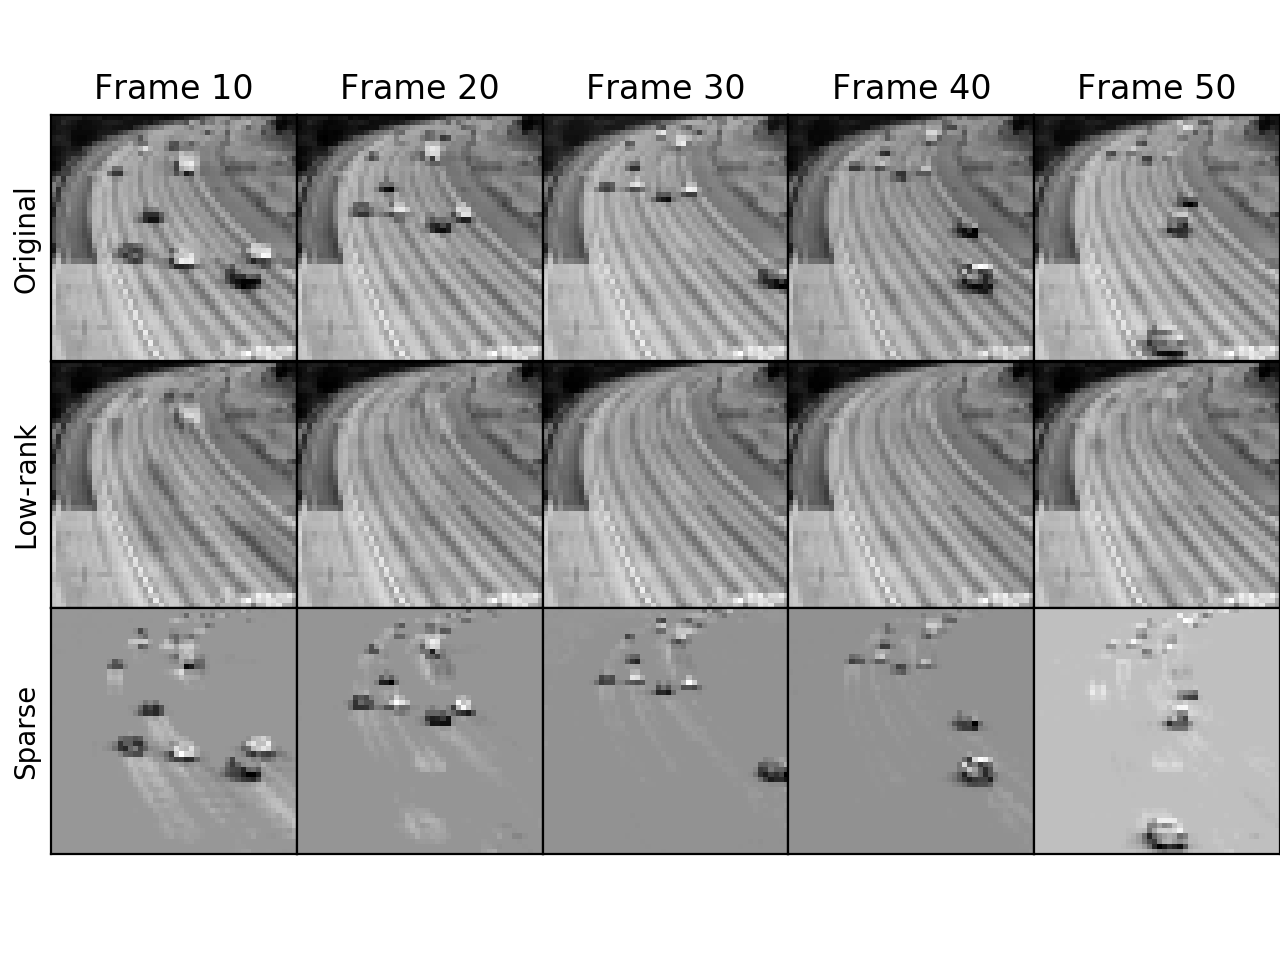
\includegraphics[width=0.5\textwidth, keepaspectratio]{Figure_4}\label{fig:subfig4}}
\caption[]{Selected frames from online background subtraction using STOC-RPCA, Incremental FPCP}
\label{fig:subfigureExample2}
\end{figure}
We benchmarked the performance of the online RPCA algorithms by running them on the dataset used in [14] and visually inspecting the results. We present some of the decompositions using both STOC-RPCA and Incremental Fast PCP on the highway dataset, at intervals of 10 frames. As expected, we observe in both cases that the low-rank/sparse decomposition improves as more frames are fed into the matrix. Based solely on the visuals, it appears that STOC-RPCA is able to converge on a better decomposition than Incremental Fast PCP can. This is borne out by the presence of more artifacts at the places where cars should be, in the low-rank component of Incremental Fast PCP as compared to that of STOC-RPCA. We also notice trails behind the moving vehicles that are extracted into the sparse component in Incremental Fast PCP that are not always present in STOC-RPCA. This suggests that STOC-RPCA converges onto a better decomposition.\newline
\begin{figure}[ht]
\centering
\subfloat[Decomposition error over number of frames]{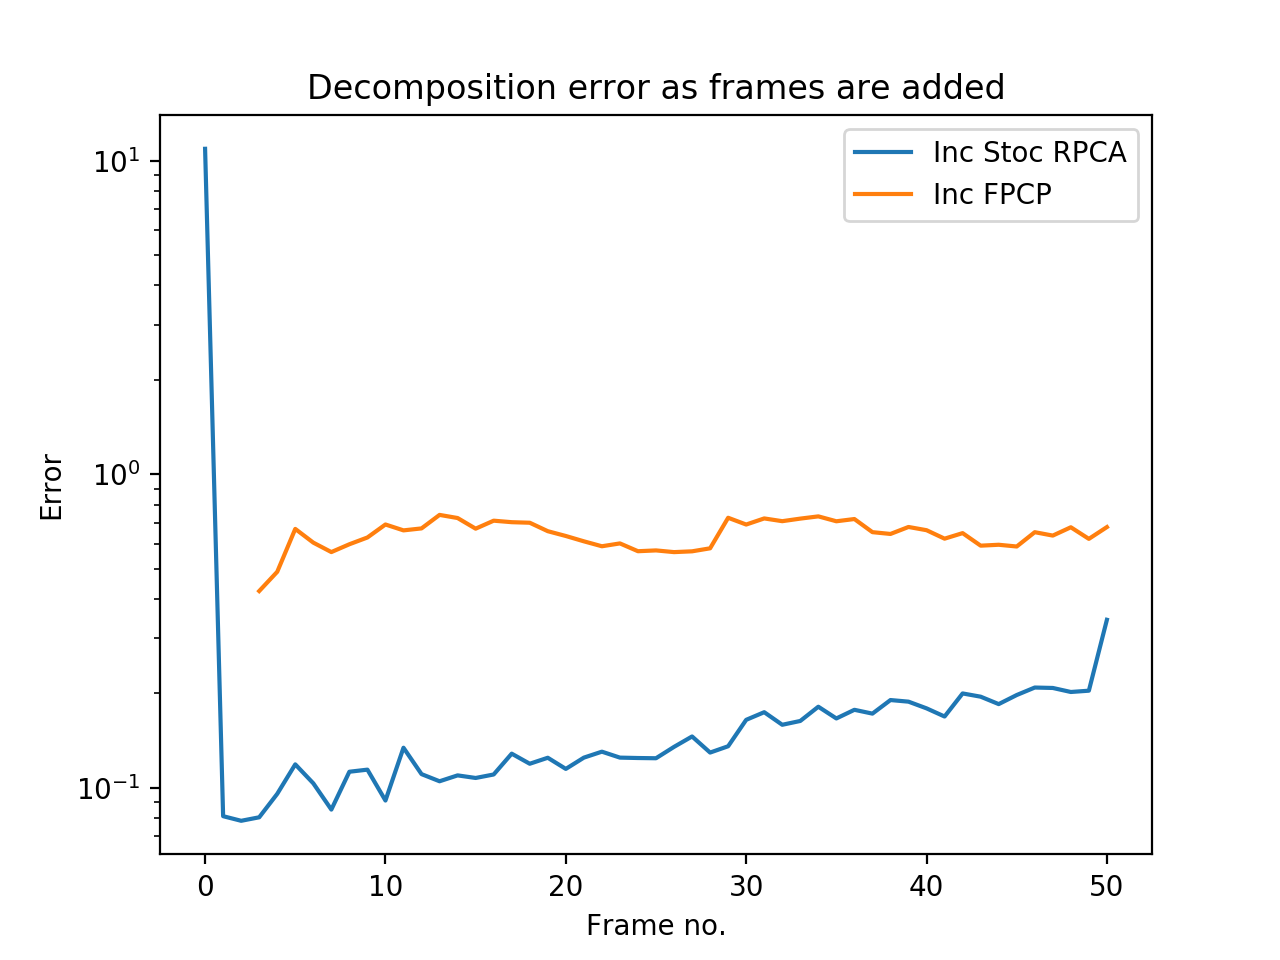
\includegraphics[width=0.45\textwidth, keepaspectratio]{Figure_5a}\label{fig:subfig5}}
\subfloat[STOC-RPCA error over iterations]{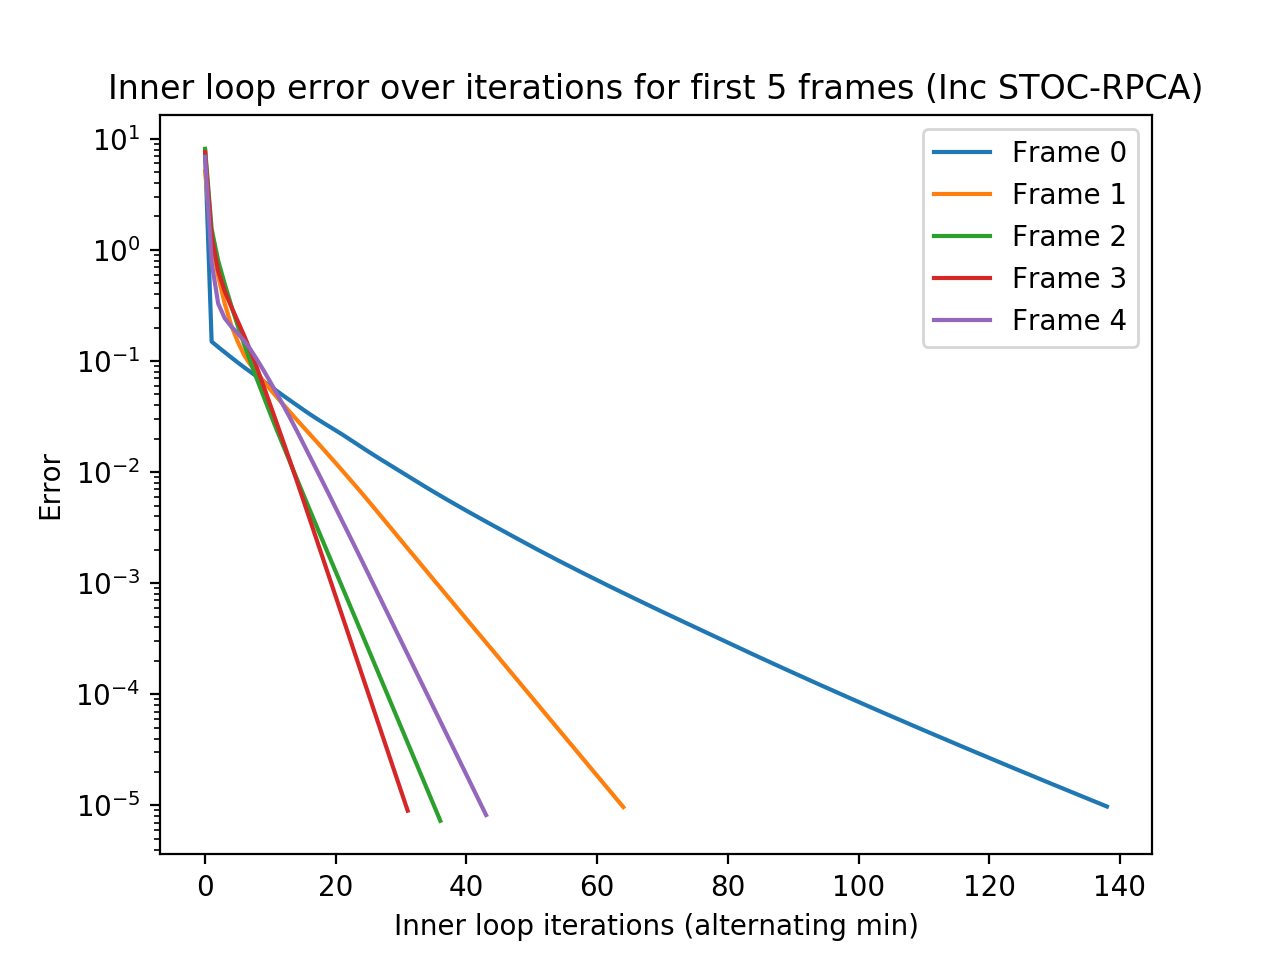
\includegraphics[width=0.45\textwidth, keepaspectratio]{Figure_6a}\label{fig:subfig6}}
\caption[]{Performance of offline RPCA algorithms on image/video processing}
\label{fig:subfigureExample3}
\end{figure}
\clearpage
The results in Fig. 1.3 appear to support the conjecture that STOC-RPCA yields a better decomposition. Fig 1.3(a) represents the decomposition error $\lVert M-L_{k}-S_{k}\rVert_{F}$ after the $k$th frame has been added to the matrix. We observe that STOC-RPCA has consistently lower error than Incremental Fast PCP in general, suggesting the $L+S$ is closer to the original $M$ with STOC-RPCA than with Incremental Fast PCP. In this sense, STOC-RPCA produces a better decomposition. The large drop in error for STOC-RPCA at the beginning occurs because $L, S$ are randomly initialized in STOC-RPCA while Incremental Fast PCP is initialized using the decomposition of the first few frames. Hence, STOC-RPCA starts off with a much larger error than Incremental Fast PCP does. This is also borne out in Fig 1.3(b), which demonstrates that far more iterations of the alternating minimization in STOC-RPCA are needed to reach convergence for the very first frame with randomly initialized $L, S$, than for the later frames which have relatively close estimates of $L,S$ from earlier frames.\newline\newline

\begin{figure}[ht]
\centering
\subfloat[Runtime for each update]{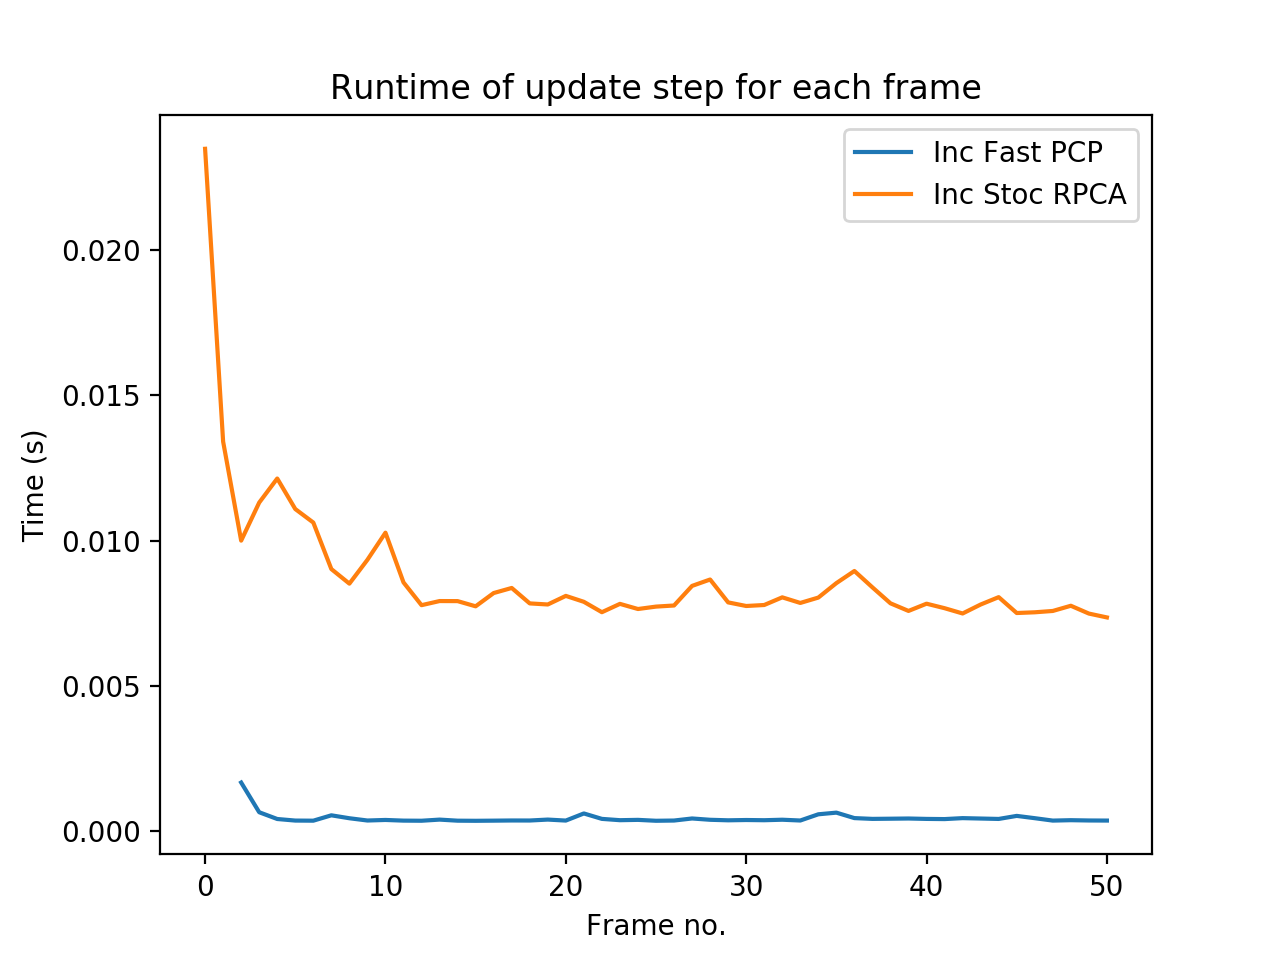
\includegraphics[width=0.5\textwidth, keepaspectratio]{Figure_7}\label{fig:subfig7}}
\subfloat[Realtime background subtraction with Incremental Fast PCP]{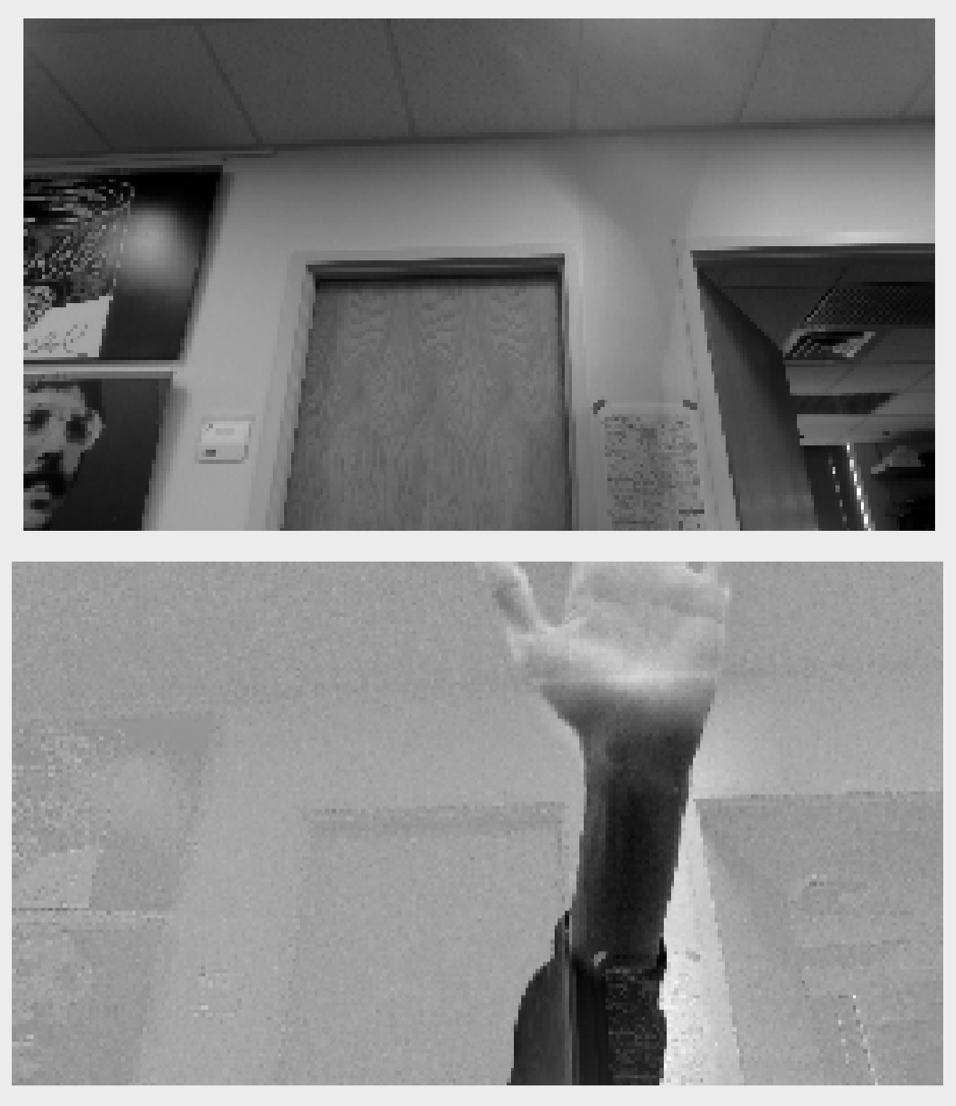
\includegraphics[width=0.3\textwidth, keepaspectratio]{Figure_8}\label{fig:subfig8}}
\caption[]{Performance of offline RPCA algorithms on image/video processing}
\end{figure}
While STOC-RPCA may yield a better decomposition that is closer to the original image than Incremental Fast PCP, Incremental Fast PCP is clearly the faster algorithm. STOC-RPCA involves an alternating minimization procedure and coordinate descent at each update (i.e. each time a new frame appears). However, Incremental Fast PCP only requires a low-rank partial SVD with a few iterations of alternating minimization to improve the estimate of $L_{k}, S_{k}$. Experimentally, we have determined that we can obtain good results with Incremental Fast PCP when we use ranks as low as 1-3 and as few as 3-4 iterations of alternating minimization. As a result Incremental Fast PCP is exceedingly fast, and as shown in Fig 1.4(a), each update step for Incremental Fast PCP runs much faster than an update step for STOC-RPCA. The efficiency of Incremental Fast PCP allowed us to implement a realtime background subtraction application, with some results demonstrated in Fig 1.4(b). There are some ghosting effects, which are particularly evident in the sparse matrix, most likely due to the fact that the camera was not perfectly stable and was shaking slightly. Stabilization of the camera and perhaps more aggressive downdating of matrix might be able to help mitigate such ghosting.

\section{Conclusions}


\iffalse

\section{References}
[1] \hspace*{8pt} E. Candes, X. Li, Y. Ma, and J. Wright, "Robust principal component analysis?," Journal of the ACM, vol. 58,
no. 3, May 2011.

[2] \hspace*{8pt}Online Robust PCA via Stochastic Optimization	(Feng, Xu and Yan, 2013). Reference: Feng, Jiashi, Huan Xu, and Shuicheng Yan. "Online robust pca via stochastic optimization." Advances in Neural Information Processing Systems. 2013.

[3] \hspace*{8pt}P. Rodriguez and B. Wohlberg, "Fast principal component pursuit via alternating minimization," in IEEE ICIP, Melbourne, Australia, Sep. 2013, pp. 69–73.

[4] \hspace*{8pt}Guyon, C., Bouwmans, T., and Zahzah, E. (2012). Robust Principal Component Analysis for Background Subtraction: Systematic Evaluation and Comparative Analysis.

[5] \hspace*{8pt}Lin, Z., Ganesh, A., Wright, J., Wu, L., Chen, M., and Ma, Y. (2009). Fast convex optimization algorithms for exact recovery of a corrupted low-rank matrix. Intl. Workshop on Comp. Adv. in Multi-Sensor Adapt. Processing, Aruba, Dutch Antilles.

[6] \hspace*{8pt}Jian L.,  Leow W.K., Sim T. (2015). Incremental Fixed-Rank Robust PCA for Video Background Recovery

[7] \hspace*{8pt} Zha H., Horst D. Simon (1999). On Updating Problems in Latent Semantic Indexing

[8] \hspace*{8pt} Lin Z., Chen M., Ma Y. (2010) The Augmented Lagrange Multiplier Method for Exact Recovery of Corrupted Low-Rank Matrices

[9] \hspace*{8pt} Cai J., Candes E., Shen Z. (2010) A singular value thresholding algorithm for matrix completion.

[10] \hspace*{8pt} Rodriguez P., Wohlberg B., (2015) Incremental Principal Component Pursuit for Video Background Modelling.

[11] \hspace*{8pt} R. Basri and D. Jacobs, Lambertian reflectance and linear subspaces.
IEEE Transactions on Pattern Analysis and Machine Intelligence,
vol. 25, no. 2, pp. 218–233, 2003

[12] \hspace*{8pt} A. Georghiades, D. Kriegman, and P. Belhumeur. From few
to many: Illumination cone models for face recognition under
variable lighting and pose, IEEE Transactions on Pattern A

[13] \hspace*{8pt} Brand, M. Fast low-rank modifications of the thin singular
value decomposition. Linear Algebra and its Applications
415(1), 20 – 30 (2006)

[14] Li, L., Huang, W., Gu, I., Tian, Q. Statistical modeling of complex backgrounds
for foreground object detection. IEEE Transaction on Image Processing (2004)
1459–1472

\fi


\end{document}

